\section{A non-additive codebook effect on scientific evidence}
\label{sec:scifact3-codebook}
The three-class SciFact diagnostic supplies a deliberately different domain
for the orthogonal control in Section~\ref{sec:codebook}. We use the same 180
frozen claim--cited-abstract pairs, with 60 cases per operational label and
one selected pair per source claim and document. The already observed base
and ordinary joint-reversal outputs are reused by hash; display-only and
code-only cells were frozen before their own inference. All four prompts
were audited, including exact tokenizer-token equality of the reused cells
with their historical records. New inference matches the original batch
size four, checkpoint, chat template and code-likelihood adapter. This is
an exploratory missing-cell follow-up, not a wholly prospective discovery
or a test of retrieval.

\begin{figure}[!ht]
\centering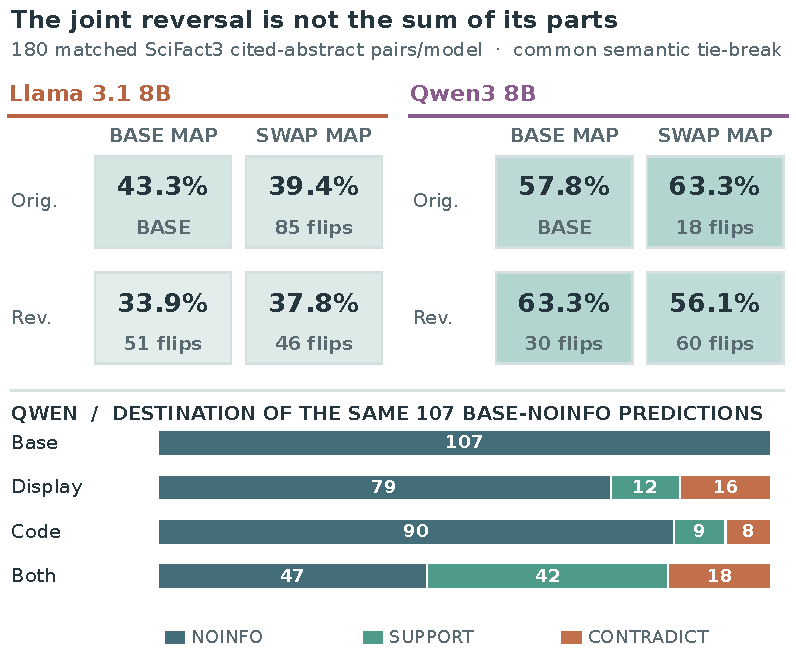
\includegraphics[width=.99\linewidth]{figures/fig_scifact3_codebook.pdf}
\caption{SciFact3 orthogonal display-order $\times$ label-to-code diagnostic
on 180 matched cited-abstract pairs per model. The grid gives accuracy and
semantic prediction flips from each model's base under a common semantic
tie-break; old native outputs remain unchanged. The lower bars follow the
\emph{same 107 cases} that Qwen predicts NOINFO at base, partitioned by
their destination class in the other cells. Both factors together have a
non-additive effect on this pinned model--adapter system; the figure does
not identify a neural mechanism. NOINFO means no annotated abstract evidence
for a cited paper, not no evidence anywhere.}
\label{fig:scifact3-codebook}
\end{figure}

Figure~\ref{fig:scifact3-codebook} makes the masking of class-level change
visible. Qwen is correct on $104/180$ base pairs, $114/180$ in either
single-factor cell, and $101/180$ under the ordinary joint reversal.
Display-only and code-only change 30 and 18 base predictions, respectively,
but the joint intervention changes 60. Both single factors gain $+5.6$
accuracy points; their combination loses $-1.7$ points, for an accuracy
difference-in-differences of $-12.8$ points (pointwise 95\% paired
source-claim-cluster interval $[-19.4,-6.1]$; 10,000 draws). The 60 joint
flips \emph{all} depart from the 107 cases Qwen labels NOINFO at base:
display-only retains 79 as NOINFO and sends 12 to SUPPORT/16 to CONTRADICT;
code-only retains 90 and sends 9/8; both retains only 47 and sends 42/18.
Among 60 reference-NOINFO pairs, Qwen's correct counts are
$54/48/52/30$ across base/display/code/both; among 60 reference-CONTRADICT
pairs they are $5/18/12/18$. Thus some migration repairs contradiction
errors while a larger joint migration also creates positive predictions on
NOINFO-reference pairs. Neither display nor code assignment alone explains the full
ordinary reversal effect. The corresponding legal single-factor flip counts
are 36/144 and 10/144 for Qwen; this cross-domain contrast is descriptive,
because source selection, label semantics and task wording differ.

Llama's native accuracy grid is $78/61/71/69$ of 180, with 51/85/42
base-relative label flips. Historical joint reversal also changes the
decoder's first-maximum tie priority. Exact top-logit ties occur in
Llama's base/display/code/both cells $6/1/11/6$ times and Qwen's
$1/6/1/0$ times. Re-decoding the stored semantic probabilities with a
fixed SUPPORT--CONTRADICT--NOINFO priority changes only six Llama joint
predictions: its common-tie grid is $78/61/71/68$, with 51/85/46 flips.
Qwen's native and common-tie four-cell results are identical, so its
non-additivity is not a tie-breaking artifact. The historical exact-repeat
controls have zero flips; all 720 new cell decisions are valid. We retain
the native records as primary historical outputs and interpret the 2$\times$2
prompt/code contrast under the fixed decoder rule. The selected pairs are
class-balanced and the NOINFO reference is derived from absent annotated
\emph{abstract} evidence for a cited document; the pointwise intervals do
not describe SciFact's natural prevalence or end-to-end fact-checking.
\FloatBarrier
